\section{Introduction}

Deep neural networks have been successfully applied to various natural language processing tasks,
%where end-to-end training become a primary option.
and as the design of neural networks evolve, there is a clear trend of increasing model complexity both in term of the architecture and the parameters count. 
%
While the expressiveness of these models help improve the prediction performance, there is a fundamental lack of interpretability that lead many to consider neural network models black boxes. 
%
Despite the difficulties, interpreting the model internals and reason about predictions are essential for understanding limitation of the model and improve upon the existing designs.

%Without understanding the background meaning that features carry, visualization relies
%on proper quantification analysis (cite). Such analysis is not easy to come up with,
%and is tied to specific task (cite).

Recently, attention networks have become a widely-adopted mechanism \cite{VaswaniShazeerParmar2017, Parikh2016}, the attention not only improves the model performance, but also yields interpretable intermediate representations (e.g. alignment among words). As a result, attention has been used as a natural interface for analyzing the internals of neural networks. Conduct analysis directly on the raw attention values can be challenging for human user, therefore, visual representations that highlight word alignments between sentences have been adopted, such as bipartite graph and heat map of the attention matrix~\cite{LiChenHovy2015, li2016understanding, lee2017interactive}.  However, many challenges remains. Firstly, for some NLP tasks, the word sequence pair among which the attentions are computed can be highly asymmetrical (i.e., in machine comprehension, the context paragraph can be much longer than the question sentence), where the standard visual encoding can not adequately handle.  In addition, many previous works present the attention in a statics setting. Yet, the ability to provide an interactive environment, where the user can instantaneously look at how changes in the input will affect the attention, and how small changes in attention will affect the prediction are crucial for interpreting the model. Finally, many previous visualization efforts, despite reveal many interesting results, focus more on illustrating potentially useful visualization technique than provide a flexible software tool that can be easily integrated into existing code base. As a result, applying these proposed techniques to real word examples may involving substantial engineering effort than many user may not afford to undertake.

To address these challenges in interpreting attention-based models, 
we introduce a flexible python library that allow user to easily generate a web-based interactive visual analytics environment for various usage via a composable visualization component design.
%
To facilitate exploratory analysis (see Figure~\ref{fig:modelPipeline}), we adopted a fully interactive pipeline, where the user can perturb the input text (via two perturbation schemes discussed in Section~\ref{sec:perturb}) and observe the effects on attention and prediction, or modify the attention to understand how it affect the predictions.
%
We demonstrate our system on two primary NLP tasks: natural language
inference (NLI) and machine comprehension (MC). For the NLI task, we visualize
decomposable attention networks which represents a series of strongly performing models \cite{Parikh2016}.
For the MC task, we present your visualization methods on bidirectional attention flow model,
which also represents a line of state-of-the-art models \cite{Seo2016}.

\begin{figure}[htbp]
\centering
\vspace{-2mm}
 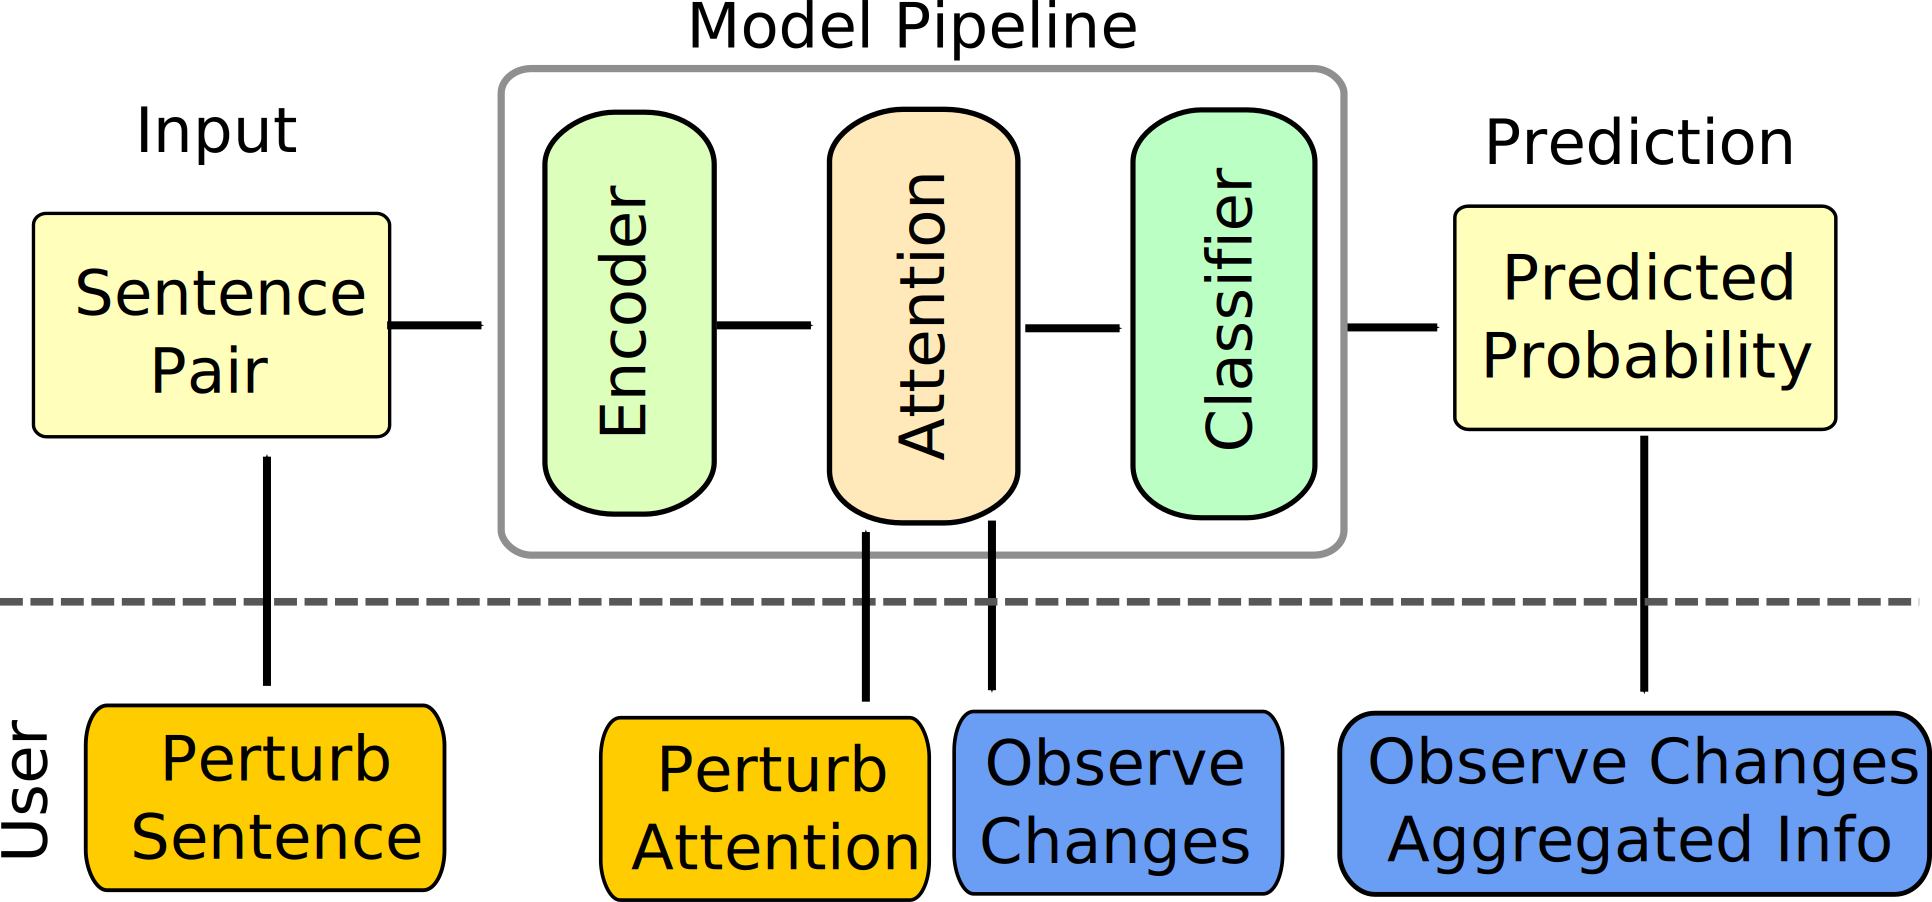
\includegraphics[width=1.0\linewidth]{pipeline}
 \vspace{-3mm}
 \caption{
 Perturbation-driven interrogation of the end-to-end models that follows the encoder, attention, and classifier structure. The user can generate small perturbation of the input (i.e., replacing synonyms, paraphrasing)
 }
 \vspace{-3mm}
\label{fig:modelPipeline}
\end{figure}

%In summary, our key contributions are:
%\begin{itemize}
%	\item Introduce an flexible visualization system for creating customized interactive visual analytic environment for attention centric neural networks models;
%	\item Illustrate the importance of envire
%	\item Demonstrate our system on two major NLP tasks with strong-performing
%	models. We observe functional limitations of these models which can be helpful
%	for future improvement on modeling.
%\end{itemize}

